\chapter{Development Process}\label{chap:developmentprocess}

\textcolor{orange}{NOE TEKST}

\section{Code Repositories}

% Github Organization and repos
All code and project-related resources are stored on GitHub under a dedicated organization\footnote{\url{https://github.com/skogkursbachelor}}. Each component of the system, as well as supporting documentation, is maintained in its own repository. This modular structure facilitates collaboration and version control throughout the development process.

An overview of the repositories and their respective purposes is shown in \autoref{tab:githubrepositories}.

\begin{table}[h]
    \centering
    \begin{tabular}{l|l}
        \hline
        \textbf{Repository} & \textbf{Description} \\
        \hline
        server & The code for the backend server. \\
        website & The code for the website. \\
        \hline
        meetingminutes & Collection of meeting minutes. \\
        diagrams & Collection of draw.io\tablefootnote{\url{https://www.drawio.com/}} diagrams. \\
        \hline
        thesis & A backup version of the thesis. \\
        projectplan & A backup version of the project plan. \\
        \hline
    \end{tabular}
    \caption[Overview of GitHub repositories]{Overview of GitHub repositories\tablefootnote{\url{https://github.com/orgs/skogkursbachelor/repositories}}}
    \label{tab:githubrepositories}
\end{table}

\section{Backup Server}

Blabla found in \autoref{lst:backupserverls}.

\begin{figure}[h]
\lstinputlisting[
    caption={Files on the backup server},
    label=lst:backupserverls,
    language=bash
]{listings/backupserver.txt}
\end{figure}

\textcolor{orange}{
Refere til 3-2-1 backup strategy hvis vi skriver om det her, hvertfall i project plan \\ \\
Hvordan det blir deployed \\ \\
Hvordan backupene skjer, crontab + git
}

\section{Time Tracking}

All project work was tracked using the self-hosted time tracking service Traggo\footnote{\url{https://traggo.net/}}. Traggo tracks work by tags making it easy to get an overview of time spent on different tasks.

\begin{table}[h]
    \centering
    \begin{tabular}{c|c|c|c}
        \hline
        \textbf{Month} & \textbf{Bjørnsen} & \textbf{Houmb} & \textbf{Total} \\
        \hline
        January  & 61h 39m  & 62h 58m  & 124h 37m \\
        February & 80h 6m   & 79h 17m  & 159h 24m \\
        March    & 88h 4m   & 88h 20m  & 176h 24m \\
        April    & 99h 40m  & 102h 38m  & 202h 18m \\
        May      &        &        &        \\
        \hline
        Total & & & \\
        \hline
    \end{tabular}
    \caption{Tracked time by month and group member}
    \label{tab:timetrackedbymember}
\end{table}

% Skriv mer om time fordeling, f.eks. hvorfor mer timer i mars enn januar etc.
\autoref{tab:timetrackedbymember} shows the total time of work for each month by the two members.

% KANSKJE IKKE TA SKJERMBILDE, LAG HELLER CHART MED LATEX f.eks. (pfg-pie).
\begin{figure}[h]
    \centering
    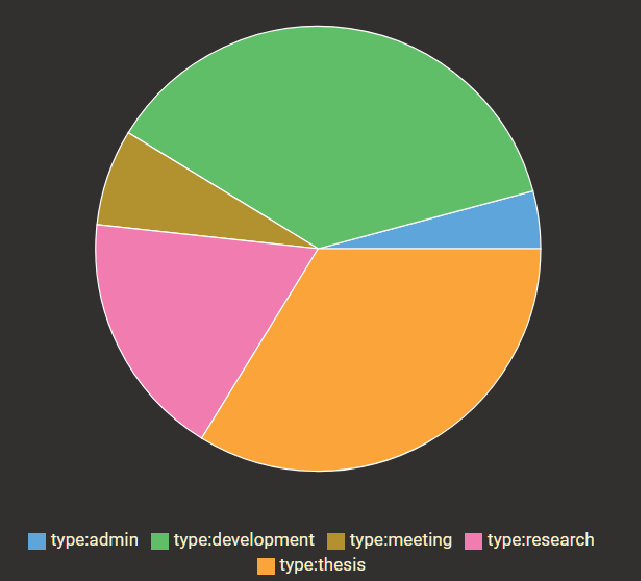
\includegraphics[width=0.5\linewidth]{figures/time_tracking_by_type.pdf}
    \caption{Pie chart of time spent in total per work type}
    \label{fig:time_tracking_by_type}
\end{figure}

% SKRIV OM TIDSFORDELING FOR DE FORSKJELLIGE OPPGAVENE (THESIS, DEV, osv.)

\section{Work Allocation}

\textcolor{orange}{Kanskje ta dette med? Hvordan utviklingsjobben for forskjellige deler av system ble tildelt?}

\section{Gantt Diagram}

A Gantt chart was created, highlighting the different sprints and key milestones. It served as a high-level plan to structure the project's progression but was not intended to be followed rigidly, allowing for flexibility and adjustments along the way, which is particularly important in agile development projects. This approach provided a clear visual overview for team coordination and progress tracking. A more detailed table of all dates referenced in the Gantt chart can be found in the project plan (see \autoref{appendix:project_plan}).

\begin{figure}[h]
    \centering
        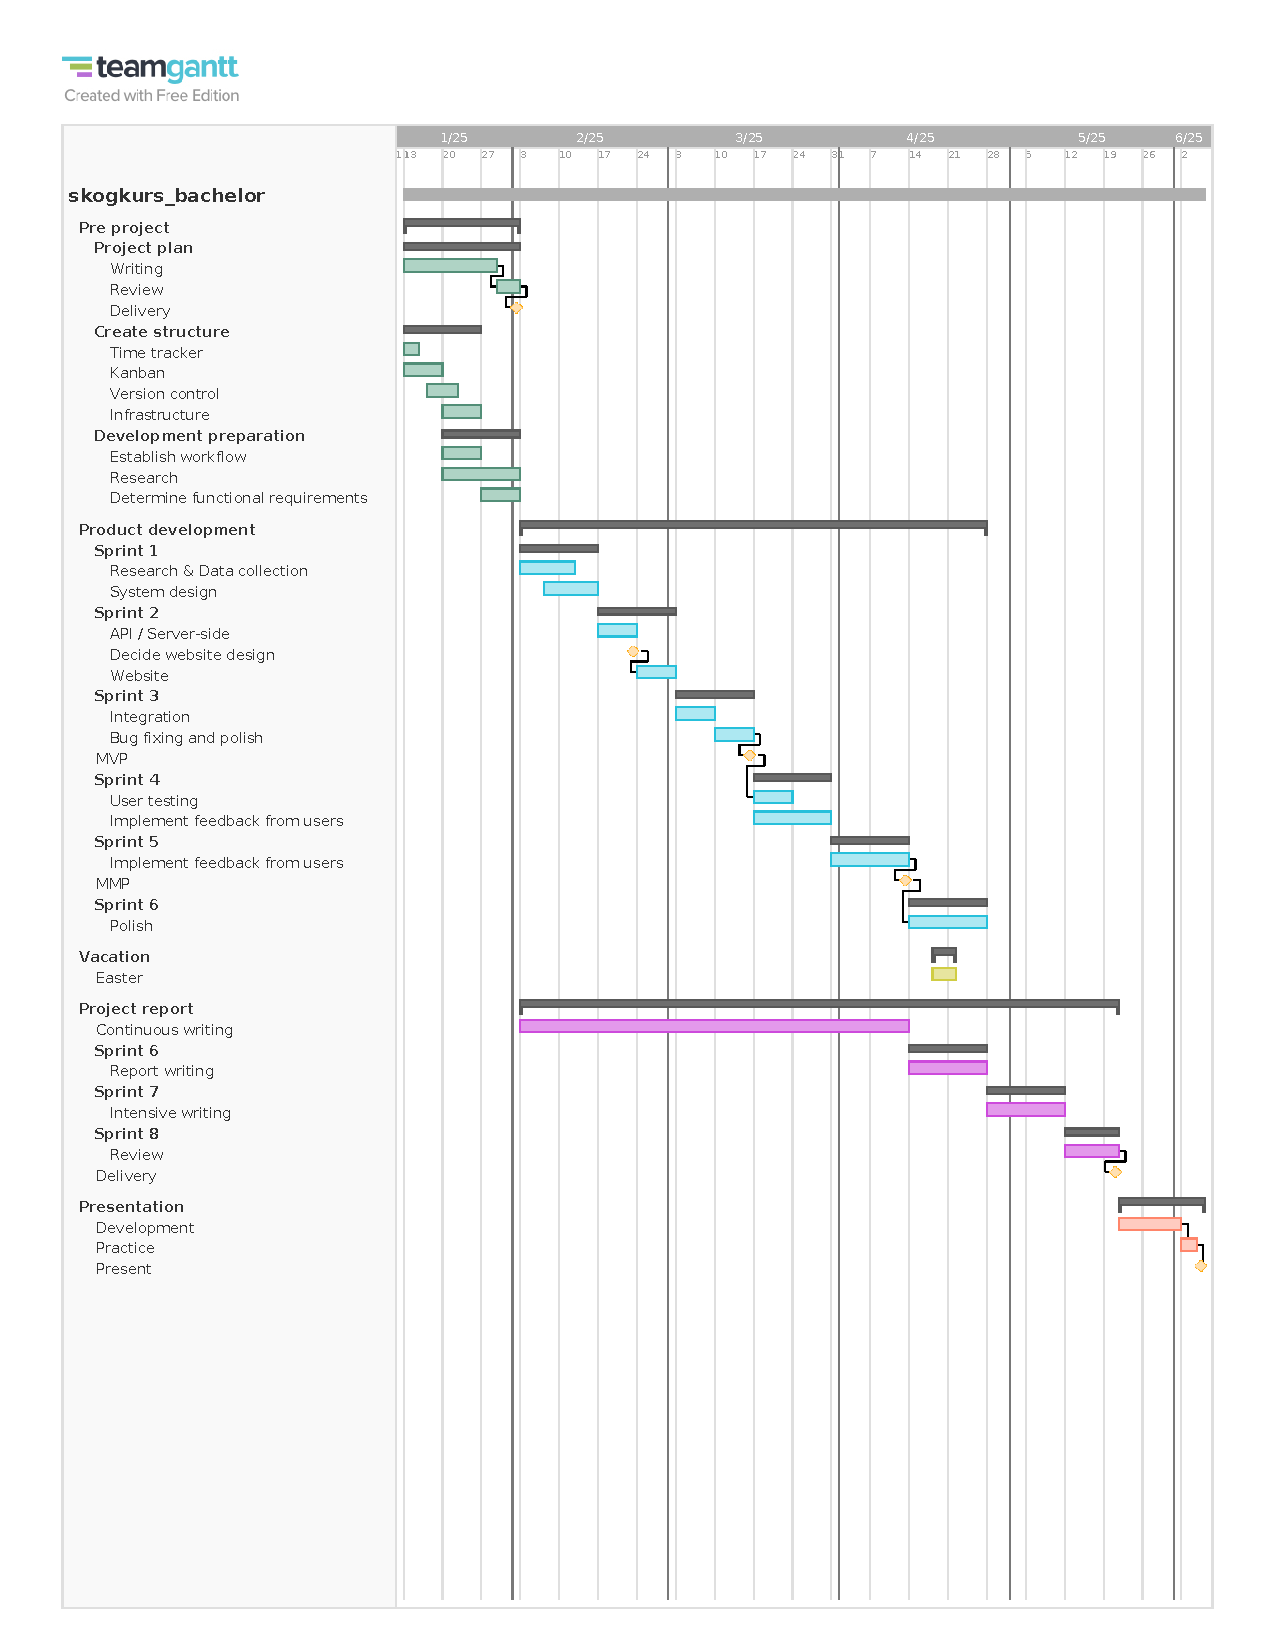
\includegraphics[width=1.0\linewidth, trim=0 60mm 0 20mm, clip]{figures/skogkurs_bachelor_gantt.pdf}
    \caption{Gantt diagram of the project}
    \label{fig:gantt_diagram}
\end{figure}

\section{Software Development Lifecycle Model}

For this project, the team needed to select an appropriate \acrfull{sdlc} model. Key factors considered in this decision included the clarity and flexibility of the requirements, team size, project timeline, product delivery goals, and prior experience \cite{sdlc_model}. 

The requirements provided by the Product Owner are intentionally ambiguous and flexible, allowing the team to prioritize the few fixed requirements upfront while iteratively refining the flexible ones over time. The team is composed of two members with similar experience levels, enabling close collaboration and effective decision-making. With a short project timeline of four months, a structure of 2-week sprints aligns perfectly with Scrum's iterative and adaptive approach, ensuring steady progress and regular opportunities for feedback. 

Given the absence of clearly defined requirements and the need for continuous collaboration with the Product Owner, the Scrum methodology was the most appropriate framework for managing the team’s workflow and project development. Traditional methodologies like Waterfall are not suitable, as they rely on fixed requirements and a linear development process, which would limit the teams flexibility \cite{waterfall_model_enwiki:1275499744}. Extreme Programming (XP), while valuable for high-collaboration environments with strict engineering practices like pair programming and test-driven development, is not fully suitable as the project does not emphasize these practices to the same extent \cite{extreme_programming}. Similarly, Lean development focuses on minimizing waste and maximizing efficiency but is less structured in terms of iterative planning, which is needed to manage evolving requirements effectively \cite{lean_programming}. By adopting Scrum, the team can iteratively refine requirements and adapt to changes throughout development \cite{sdlc_model}. To implement Scrum effectively, several key practices are integrated into our workflow \cite{scrum_guide}.

\begin{itemize}
    \item \textbf{Sprint Meetings:} The project is divided into 2-week sprints. At the start of each sprint, sprint meetings included sprint planning, reviews, and retrospectives. During the planning phase, the team selects tasks from the product backlog to form the sprint backlog for the upcoming sprint. The review phase focuses on evaluating progress and determining whether adjustments to the product backlog are needed. The goal of the retrospective phase is to identify areas for improvement in the Scrum process itself.
    \item \textbf{Daily Scrum Meetings:} Short daily meetings are conducted to discuss the progress of ongoing tasks, identify potential obstacles, and ensure alignment between team members. 
    \item \textbf{Scrum Master:} Given that the team consists of only two members, we have decided to share the role of Scrum Master. Both members are responsible for ensuring adherence to the Scrum framework and continuously working to improve team efficiency. This collaborative approach allows us to maintain flexibility while upholding Scrum principles throughout the project.
    \item \textbf{Kanban:} To complement Scrum and further enhance workflow visibility, a Kanban board is utilized to track and manage tasks on GitHub. The Kanban board consists of columns representing different stages of the workflow, such as Product Backlog, Sprint Backlog, In Progress, In Review, Done, and Discarded.
\end{itemize}

\section{Sprints}

\textcolor{orange}{PUTTE HVERTFALL SPRINTREFERATENE I VEDLEGG, MEN KAN SKRIVE NOE OM SPRINTS. Peke til vedlegg. Sammenlign med det som står over, ta med sprint planning, reviews og retrospective. Sprint Reviews for selve produktet, retrospectives for prossessen. Lite å snakke om på retrospektive, men var en periode med lite arbeid på bachelor på grunn av annet fag (vet ikke om det skal nevnes?)}
% peke til vedlegg
% Sammenlign med det som står over, ta med sprint planning, reviews og retrospective

\textbf{Sprint 1}
\begin{itemize}
    \item Research & data collection
    \item System design
\end{itemize}

\textbf{Sprint 2}
\begin{itemize}
    \item API / Server-side
    \item Decide website design
    \item Website
\end{itemize}

\textbf{Sprint 3}
\begin{itemize}
    \item Integration
    \item Bug fixing and polish
    \item MVP
\end{itemize}

\textbf{Sprint 4}
\begin{itemize}
    \item User testing
    \item Implement feedback from users
\end{itemize}

\textbf{Sprint 5}
\begin{itemize}
    \item Implement feedback from users
    \item MMP
\end{itemize}

\textbf{Sprint 6}
\begin{itemize}
    \item Polish of code
    \item Report Writing
\end{itemize}

\textbf{Sprint 7}
\begin{itemize}
    \item Intensive writing
\end{itemize}


\textbf{Sprint 8}
\begin{itemize}
    \item Final review of the report
\end{itemize}

For more details about each sprint, the meeting minutes from each sprint meeting can be found in \autoref{appendix:sprint_meetings}.

\section{Meetings}

In addition to internal sprint meetings, the team held regular meetings with both the Supervisor and the Product Owner. Weekly meetings with the Supervisor offered opportunities to ask questions, receive technical guidance, and get constructive feedback, both on the product and the written report.

Meetings with the Product Owner were held on an as-needed basis rather than at fixed intervals. Most of these meetings were conducted digitally via Microsoft Teams. They were particularly valuable for clarifying requirements, discussing design decisions, and showcasing progress through product demos.

Minutes from all meetings with the Supervisor and the Product Owner can be found in \autoref{appendix:meeting_minutes}.

\section{Minimum Viable Product}

A Minimum Viable Product (\acrshort{mvp}) is a concept that focuses on learning about customers with minimal effort. An \acrshort{mvp} is an early version of a product designed to test whether customers will use or buy it, often taking the form of a simple prototype, landing page, or manually operated service. The key benefit of an \acrshort{mvp} is that it allows teams to validate ideas early, minimizing wasted effort on products that may not succeed \cite{agile_alliance_mvp}. 

\textcolor{orange}{BLE IKKE NOE MMP. Skrev om under litt: user testing -> reviews med PO, fjernet "Further details about the user testing process and findings are discussed in a later chapter."}

During the development of the website, we conducted reviews with the Product Owner to gain insights into how the target audience (transport managers) would interact with the product and identify any missing features or necessary improvements. For the \acrshort{mvp}, we prioritized implementing the core functionalities users would need, as illustrated in the use case diagram in \autoref{fig:use_case_diagram}.

\section{Minimum Marketable Product}

A Minimum Marketable Product (\acrshort{mmp}) is the next step after an \Gls{mvp} in product development. While an \acrshort{mvp} focuses on testing assumptions and user preferences, an MMP includes essential features that meet customer needs, provide a good user experience, and generate business value. It is designed to launch quickly with must-have functionality, avoiding unnecessary features that add complexity without value. The MMP approach involves refining the product to only what is essential for success. Typically, teams first develop \acrshort{mvp}s to gather insights, then use these findings to build an \acrshort{mmp} ready for general release. In agile development, combining \acrshort{mvp} and \acrshort{mmp}s helps streamline product evolution while minimizing risk and unnecessary work \cite{wanner_mmp}. 

The initial plan was to conduct user testing and implement the feedback given to create a \acrshort{mmp}, but due to unforeseen circumstances this would not be created. This will be discussed later in \autoref{chap:discussion}.
